% multiple1902 <multiple1902@gmail.com>
% intro.tex
% Copyright 2011~2012, multiple1902 (Weisi Dai)
% https://code.google.com/p/xjtuthesis/
%
% It is strongly recommended that you read documentations located at
%   http://code.google.com/p/xjtuthesis/wiki/Landing?tm=6
% in advance of your compilation if you have not read them before.
%
% This work may be distributed and/or modified under the
% conditions of the LaTeX Project Public License, either version 1.3
% of this license or (at your option) any later version.
% The latest version of this license is in
%   http://www.latex-project.org/lppl.txt
% and version 1.3 or later is part of all distributions of LaTeX
% version 2005/12/01 or later.
%
% This work has the LPPL maintenance status `maintained'。
%
% The Current Maintainer of this work is Weisi Dai。
%

\chapter{基于边缘骨架切割的文字检测方法}
\echapter{Text detection based on Skeleton-cut detector}
\label{sec.c3}

    边缘是一种可以很好地表征文字结构信息的特征。但是想要在自然场景图片的背景中分离出来文字边缘是一件极具困难的工作,其中最有挑战性的问题是如何解决边缘粘连(edge-adhesion)问题。针对这种边缘粘连问题,本文提出了一种基于边缘骨架切割的文字检测方法。

    \section{问题的提出}
    \esection{Questions Posed}

    基于区域和基于连通部件的文字检测方法各有优缺点。其中,基于区域方法的检测结构可在噪声环境中精准提取到文字,这是因为这些方法在图像上大多采用滑动窗进行细致的探索,并执行多尺度的处理来提取特征。但相应地就会导致分类窗口过多,计算量太大,对时间性能的要求也更高;而另一类方法的处理目标是连通部件,其数量相比滑动窗要更可控,因此处理时间大为缩短,并且其检测到的结果可直接应用到识别文字的阶段。但此类方法的问题是在曝光或低对比度环境中难以从背景中分离出连通区域,并且过于依赖图像分割算法的结果。如何对这两类方法折衷,以在保证精准的文字检测效果的同时还能达到较高的效率,是一个值得深入研究的问题。

    在基于区域的文字检测方法中主要有基于MSER 和基于边缘的这两类主流方法。MSER 类方法存在的问题有:当文字位于玻璃、浮雕等反光物体的表面时将无法作为极值区域被提取出来;采用ER树生成候选的文字区域会导致重复、嵌套和计算量过大等问题;用来过滤ER 的启发式规则用到许多固定阈值。而基于边缘的方法对图像边缘提取的结果比较敏感,如果存在背景与文字边缘粘连问题,或不能完整提取文字边缘时,就很难进行后续的文字检测的分析,并造成漏检问题。针对上述的这些问题,一种解决办法便是利用文字自身的双边属性,而采用基于边缘的方法对此属性进行最佳的表征,然后再融合上MSER的方法来提取候选文字的感兴趣区域proposals,最后在这些proposals中进行单尺度滑动窗的变化并输入到CNN 分类器中作分类。那么其中最关键的步骤就是解决背景与文字的边缘粘连问题,以提取出完整的文字边缘。

    依据以上提出的问题及对其的分析,本文提出了一种基于边缘骨架切割的文字检测方法。首先求取场景文字图片的边缘骨架图,并在其上利用8 连通域分析方法找到文字边缘和背景边缘的粘连点。然后自适应地断开这些粘连点,并将分离开来候选文字边缘骨架段输入到两阶段的CNN分类器中作文字与非文字的判别。最后提出一种结合MSER的局部迭代优化算法来提高文字检测的准确度。

    \section{方法原理与步骤}
    \esection{Principle and Summary of The Method}

    基于边缘骨架切割的文字检测子的具体流程如图\ref{fig.c3_overview} 所示。首先对于输入的场景文字图片,利用结构化边缘检测方法\cite{Dollar2015Fast} 得到输入图片的结构化边缘响应图,如图\ref{fig.c3_overview}(b) 所示。然后基于一系列像素强度值阈值,对边缘响应图进行分割,得到相应的二值化边缘图。接着在每个二值边缘图上,通过细化操作得到其边缘骨架图,如图\ref{fig.c3_overview}(c) 所示。图中的红色结点是在边缘骨架上,通过8 领域内像素点分析所找到的边缘骨架结点。而文字边缘与背景间的粘连点,就存在于这些边缘骨架结点中。
    为了将文字边缘从背景杂质中切割出来,需要切割开这些边缘骨架结点,以解决文字边缘的粘连问题。而由不同的二值边缘图所生成的边缘骨架图上的结点是不同的。因此选择合适的边缘骨架图上的结点进行切割,是解决文字边缘粘连问题的核心步骤。

    \begin{figure*}[!h]
    \centering
    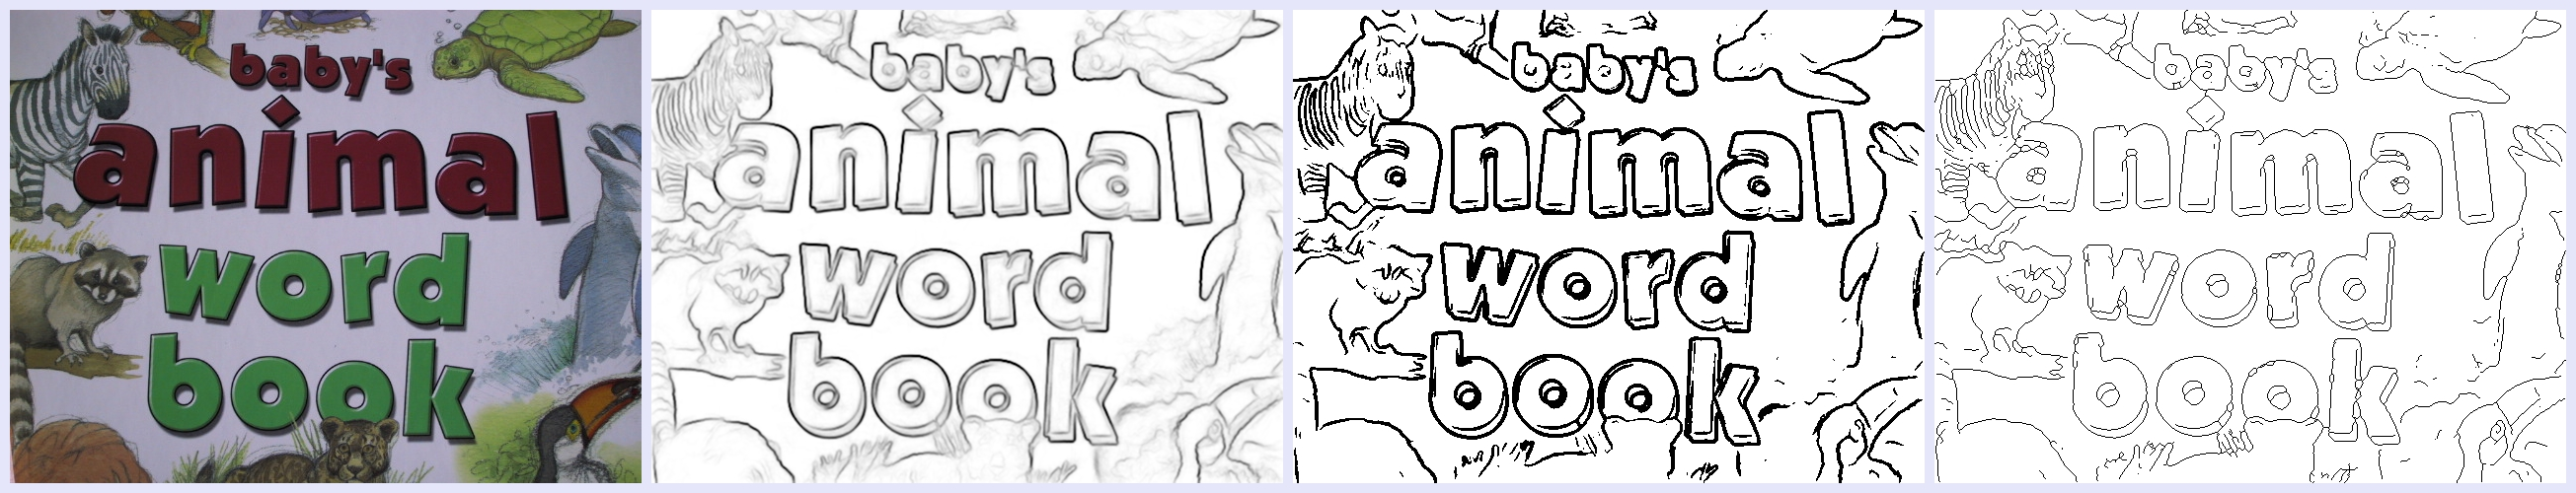
\includegraphics[width=\textwidth]{./figures/c3_overview_1.jpg}
    \begin{minipage}[t]{0.22\linewidth}
    \centerline{ \small (a) 输入场景文字图}
    \end{minipage}
    \begin{minipage}[t]{0.22\linewidth}
    \centerline{ \small (b) 边缘响应}
    \end{minipage}
    \begin{minipage}[t]{0.22\linewidth}
    \centerline{ \small (c) 边缘二值图}
    \end{minipage}
    \begin{minipage}[t]{0.22\linewidth}
    \centerline{ \small (d) 边缘骨架}
    \end{minipage}
    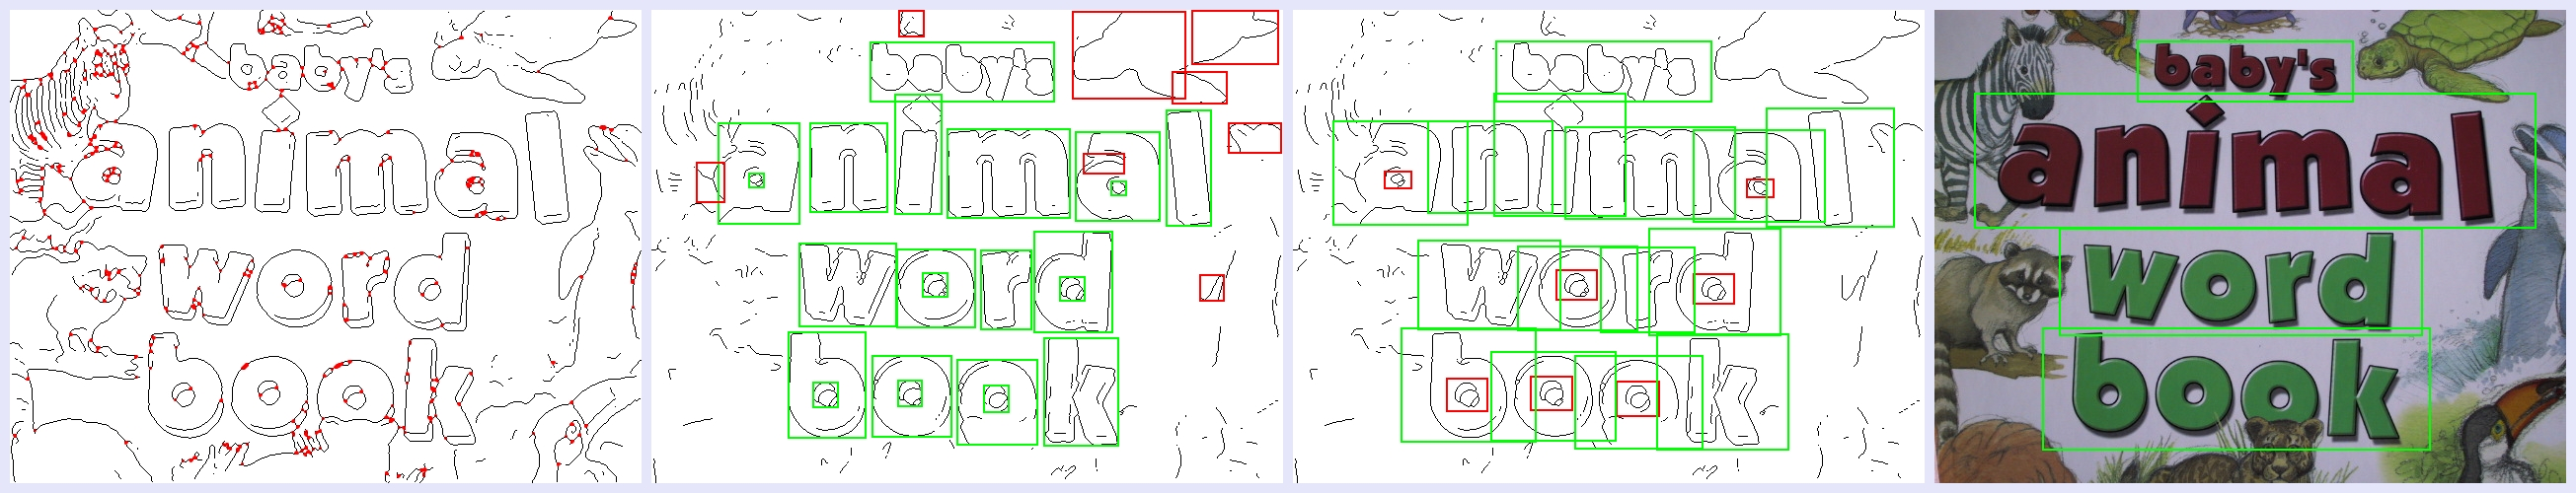
\includegraphics[width=\textwidth]{./figures/c3_overview_2.jpg}
    \begin{minipage}[t]{0.22\linewidth}
    \centerline{ \small (e) 边缘骨架切割}
    \end{minipage}
    \begin{minipage}[t]{0.22\linewidth}
    \centerline{ \small (f) 非文字骨架的滤除}
    \end{minipage}
    \begin{minipage}[t]{0.22\linewidth}
    \centerline{ \small (g) 文本行生成}
    \end{minipage}
    \begin{minipage}[t]{0.22\linewidth}
    \centerline{ \small (h) 文字粗略定位结果}
    \end{minipage}
    \caption{基于边缘骨架切割的文字检测方法的流程图}
    \label{fig.c3_overview}
    \end{figure*}

    这里通过实验观察可知,那些分割阈值较低所得的二值边缘图所生成的边缘骨架较为杂乱,更可能是无效的边缘骨架,如图\ref{fig.c3_select_skeleton}(a) 所示。
    因此这里采用欧拉数计算,来从一系列边缘骨架图中选择出最合适的边缘骨架图,欧拉数的计算过程如图\ref{fig.c3_select_skeleton}(b) 所示。在边缘骨架图中,所有的候选边缘骨架都要经过形态学滤除,以过滤掉大部分明显不是文字的边缘骨架。该滤除过程如图\ref{fig.c3_overview}(c) 到图\ref{fig.c3_overview}(d) 的变化所示。紧接着,剩余的不易区分的非文字边缘骨架,可通过基于CNN 的分类器来进一步滤除。该滤除过程如图\ref{fig.c3_overview}(d) 到图\ref{fig.c3_overview}(e) 所示,红色框中包含的不易区分的非文字边缘骨架,可通过CNN 分类器去除掉。最后如图\ref{fig.c3_overview}(f) 所示,基于非极大值抑制和文本行聚集操作,得到粗略的文本行定位结果。

    \section{文字骨架的提取与切割}
    \esection{Text skeleton's extraction and cutting}

        \subsection{文字骨架的生成}
        \esubsection{Text skeleton's construction}
        \label{sec.c3_skeleton}

        %一系列分割阈值,得到不同的二值边缘图,并生成相应的边缘骨架图;低分割阈值的二值图所生成骨架图较为杂乱,不适合用于后续的边缘骨架切割步骤;这部分内容在supplement 上有,将其作图写在skeleton 的生成一节中。

        在输入的场景文字图像上,通过结构化边缘检测子\cite{Dollar2015Fast} 得到了图像的结构化边缘响应图。边缘响应图并不是二值图,其每个位置上的像素点的值代表的是该像素点属于边缘的概率。如图\ref{fig.c3_overview}(b) 所示,某位置的像素点的值越大,图中该位置的像素点的颜色就越深,说明该位置的像素点越可能位于一条边缘之上。既然边缘响应图是每个位置像素点的值都不尽相同的概率图,为了便于观察,用图\ref{fig.c3_response_to_map} 第一行的三维图展示其概率响应。然后按照一系列像素灰度值阈值,对边缘响应图进行分割,得到相应阈值下的二值边缘图。这些二值边缘图如图\ref{fig.c3_response_to_map} 中第二行所示。

        从图\ref{fig.c3_response_to_map} 中可以看出,当分割阈值较小时,从边缘响应图上分割得到的二值边缘图较为清晰,但存在大量非文字的边缘,导致文字边缘与背景的粘连问题较为严重。而当分割阈值较大时,从边缘响应图上分割得到的二值边缘图中,大部分非文字的边缘已经被略去,而文字边缘相对而言被较为完整的保留下来,使得文字边缘的粘连问题得到缓解。但同时,大阈值分割下的二值边缘图较为模糊和残缺,边缘时有断裂现象,不利于后续的边缘分析与处理。

        \begin{figure*}[!h]
        \centering
        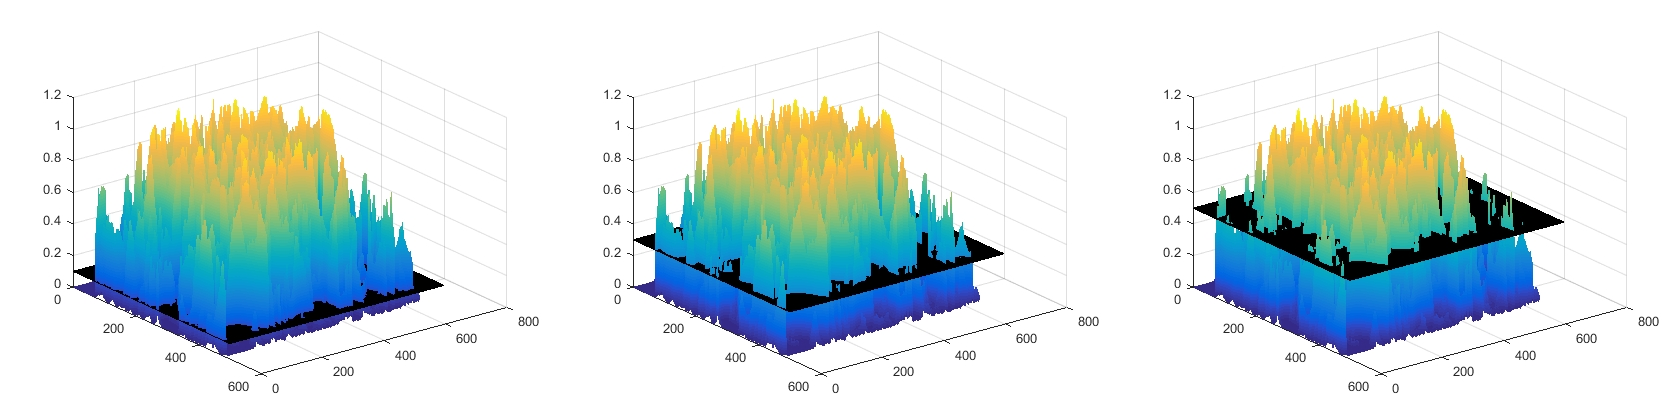
\includegraphics[width=\textwidth]{./figures/c3_edge_response.jpg}
        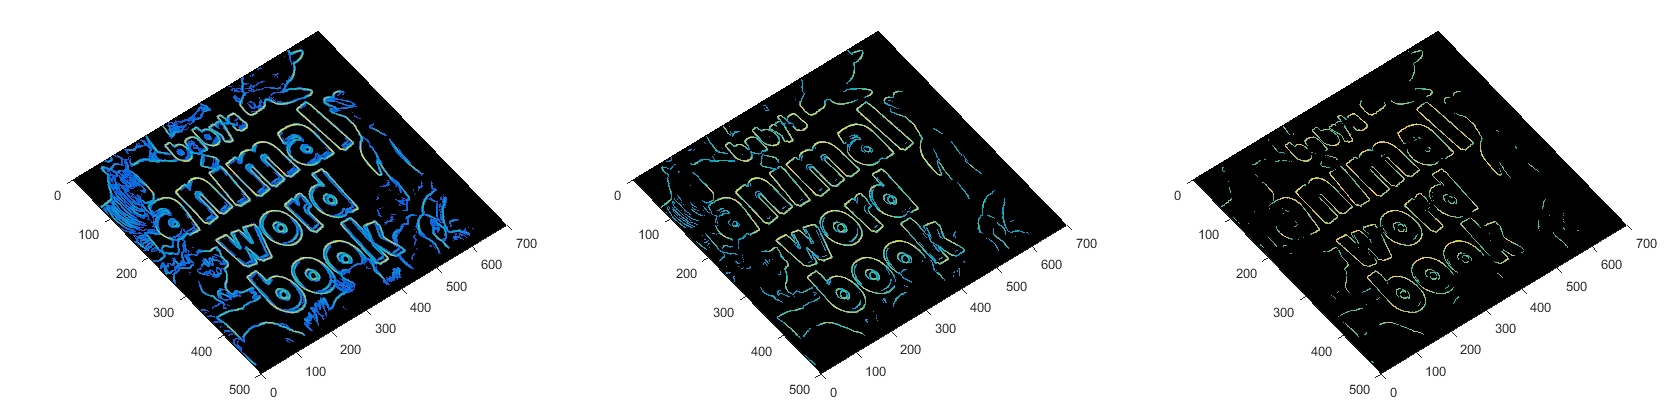
\includegraphics[width=\textwidth]{./figures/c3_edge_map.jpg}
        \begin{minipage}[t]{0.32\linewidth}
        \centerline{ \small (a) 阈值 $t = 0.1$}
        \end{minipage}
        \begin{minipage}[t]{0.32\linewidth}
        \centerline{ \small (b) 阈值 $t = 0.3$}
        \end{minipage}
        \begin{minipage}[t]{0.32\linewidth}
        \centerline{ \small (c) 阈值 $t = 0.5$}
        \end{minipage}
        \caption{在边缘响应图上通过一系列的分割阈值得到相应的边缘二值图}
        \label{fig.c3_response_to_map}
        \end{figure*}

        因此,分割阈值不同,从边缘响应图上分割得到的二值边缘图也不同。较高阈值下的边缘图保留了更多的边缘信息,但更难区别文字与非文字边缘。较低阈值的边缘图去除了非文字边缘信息,但边缘更不清晰。不同于Canny 算子\cite{Ding2001On} 等固定阈值的边缘二值图检测方法,本文采用递增的分割阈值从边缘响应图中得到一系列候选边缘二值图,然后从中自适应地选择出最合适的二值边缘图进行后续处理。自适应选择最优二值边缘图的内容会在\ref{sec.c3_skeleton_cut} 节中详细阐述。

        接下来利用8连通区域细化方法\cite{Lam2002Thinning} 在二值边缘图上提取边缘的骨架线。该细化方法会一直重复迭代操作,直到图像不再发生变化。每次迭代操作包含2个子迭代操作:在第1个子迭代操作中,当且仅当条件 $G_1$, $G_2$ 和 $G_3$ 全部满足时,二值边缘上的像素点$p$ 将被消除。而在第2个子迭代操作中,当且仅当条件$G_1$, $G_2$ 和 $G_3$$'$ 全部满足时,二值边缘上的像素点$p$ 将被消除。这些细化操作的条件如下所示:

        1)条件$G_1: X_H(p)=1$

        其中,$X_H(p)=\sum\limits_{i=1}^4b_i$,而
        $b_i=\left\{
        \begin{array}{cl}
        1, &  if \ x_{2i-1}=0 \; and \; (x_{2i}=1 \; or \; x_{2i+1}=1)\\
        0, &  otherwise.
        \end{array}
        \right.$

        2)条件$G_2: 2\le \left\{n_1(p),n_2(p)\right\} \le3$

        其中,$n_1(p)=\sum\limits_{k=1}^4x_{2k-1}\lor x_{2k}$,并且
        $n_2(p)=\sum\limits_{k=1}^4x_{2k} \lor x_{2k+1}$

        3)条件$G_3: (x_2 \lor x_3 \lor \overline{x}_8) \land x_1=0$

        4)条件$G_3$$'$$: (x_6 \lor x_7 \lor \overline{x}_4) \land x_5=0$

        细化方法将重复迭代操作,直到提取出的边缘的骨架图不再变化为止。因此候选文字骨架的生成步骤如图\ref{fig.c3_skeleton} 所示:首先利用结构化边缘检测子在输入的场景文字图像中计算得到结构化边缘响应,然后通过一系列分割阈值获得相应的二值边缘图,最后通过8 连通区域细化方法得到边缘骨架图,即宽度为1 个像素宽的边缘骨架线,如图\ref{fig.c3_skeleton}(d) 中的1 个像素宽的黑色细线所示。

        \begin{figure*}[!h]
        \centering
        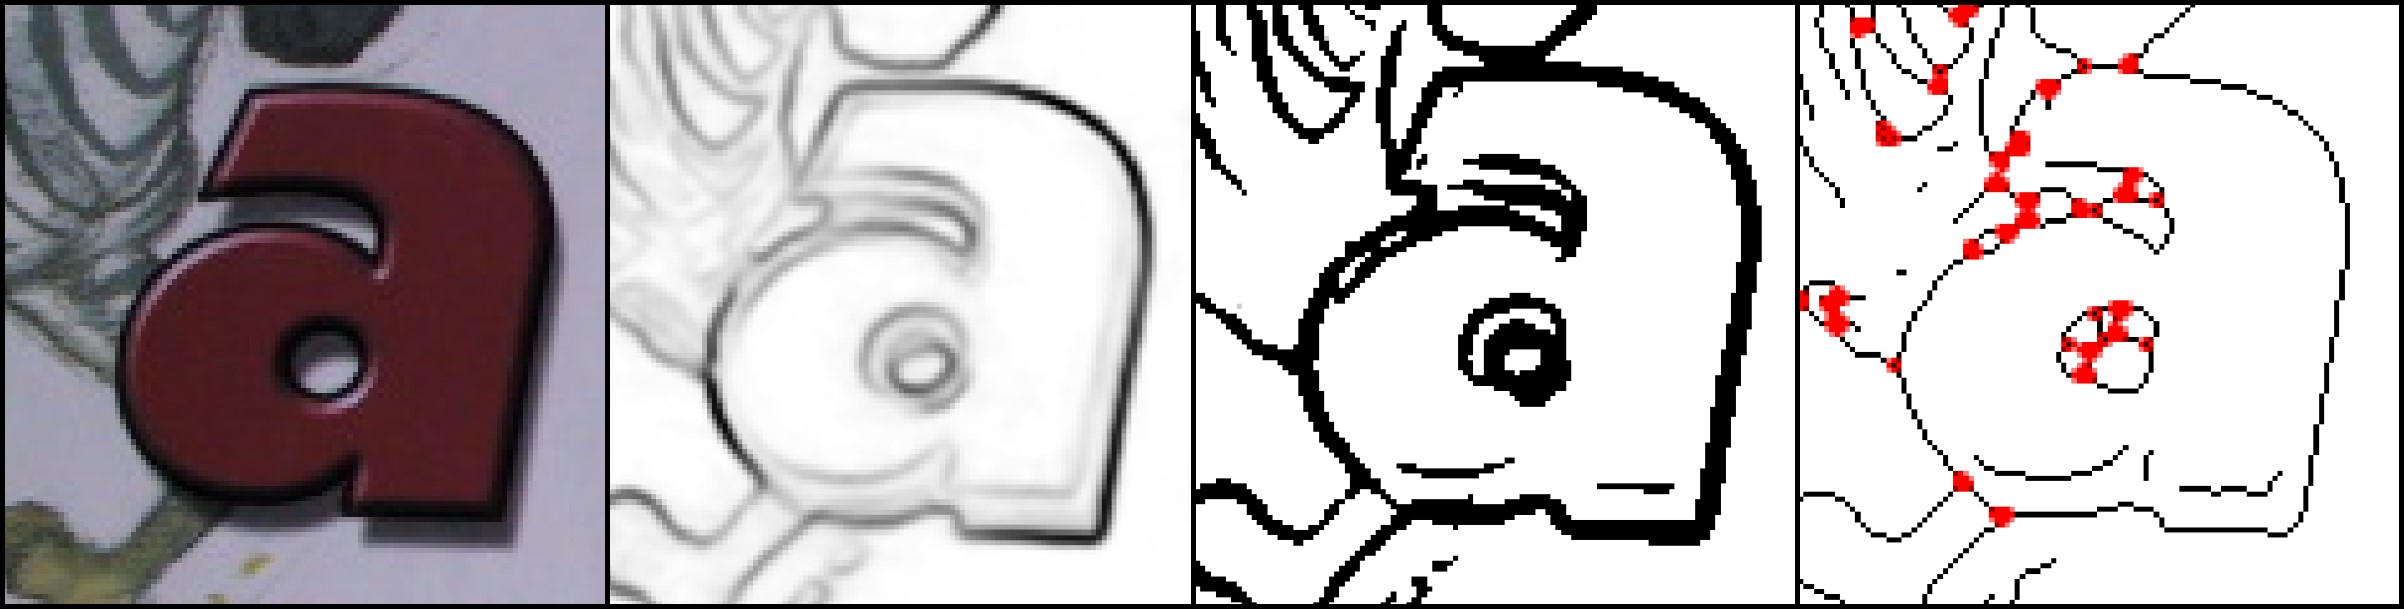
\includegraphics[width=\textwidth]{./figures/c3_skeleton.jpg}
        \begin{minipage}[t]{0.24\linewidth}
        \centerline{\small (a)原图}
        \end{minipage}
        \begin{minipage}[t]{0.24\linewidth}
        \centerline{\small (b)边缘响应}
        \end{minipage}
        \begin{minipage}[t]{0.24\linewidth}
        \centerline{\small(c) 边缘二值图}
        \end{minipage}
        \begin{minipage}[t]{0.24\linewidth}
        \centerline{\small (d)边缘骨架图}
        \end{minipage}
        \caption{文字边缘骨架生成的流程图}
        \label{fig.c3_skeleton}
        \end{figure*}

        \subsection{文字骨架粘连点的检测和切割}
        \esubsection{Text adhesion-junctions' detection and cutting}
        \label{sec.c3_skeleton_cut}

        生成边缘骨架图后,就可以通过8 连通区域的像素点数分析来检测边缘骨架粘连点。检测边缘骨架粘连点$J$ 的公式如下所示:

        \begin{equation}
        J=\left\{ p|n(p)=\sum_{k=1}^8x_k>t \right\},
        \label{eq:c3_junctions}
        \end{equation}

        在公式\ref{eq:c3_junctions} 中,$n_p$ 是像素点$p$ 的8 连通区域内像素点的数目之和,而$t$ 是用来提取粘连点的像素点数目阈值。通过实验观察,令$t = 3$ 能检测到数目合适的候选边缘骨架粘连点,如图\ref{fig.c3_skeleton} 中的红色结点所示。

        在\ref{sec.c3_skeleton} 节中已经阐述,对于边缘响应图,利用不同的分割阈值可以得到相应的二值边缘图。而且分割阈值较大时,二值边缘清晰但粘连问题严重,阈值较小时非文字边缘大部分被消除但是文字边缘也出现断裂问题。因此选择合适的二值边缘图,使得既不会在图中出现过多的背景边缘,又能提供清晰的边缘信息,对后续解决边缘粘连问题至关重要。而观察由二值边缘图所生成的边缘骨架图的形态,就是一种判断所选边缘图是否合适的方式。

        \begin{figure*}[!h]
        \centering
        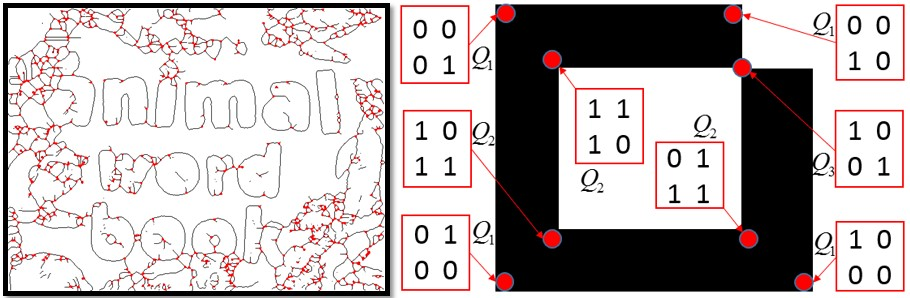
\includegraphics[width=\textwidth]{./figures/c3_select_skeleton.jpg}
        \begin{minipage}[t]{0.48\linewidth}
        \centerline{\small (a)无效的边缘骨架图}
        \end{minipage}
        \begin{minipage}[t]{0.48\linewidth}
        \centerline{\small (b)在边缘骨架图上计算欧拉数}
        \end{minipage}
        \caption{通过欧拉数的计算,选择出最合适的边缘骨架图}
        \label{fig.c3_select_skeleton}
        \end{figure*}

        如图\ref{fig.c3_select_skeleton}(a) 所示,当分割阈值偏小时,从边缘响应图上分割得到的二值边缘图中混有过多的非文字边缘信息,因此通过细化操作所得的边缘骨架图十分杂乱无序,不能作为解决边缘粘连问题的有效信息。在这种混乱的边缘骨架图上检测到的候选边缘骨架粘连点,数目特别多且分布杂乱。因此,检测到的候选边缘骨架粘连点的数目,在一定程度上可以指示所选二值边缘图和相应的边缘骨架图的合理程度。除此之外,还可以通过对生成的边缘骨架图计算欧拉数,来避免选择不合适的边缘骨架图。

        \begin{figure*}[!h]
        \centering
        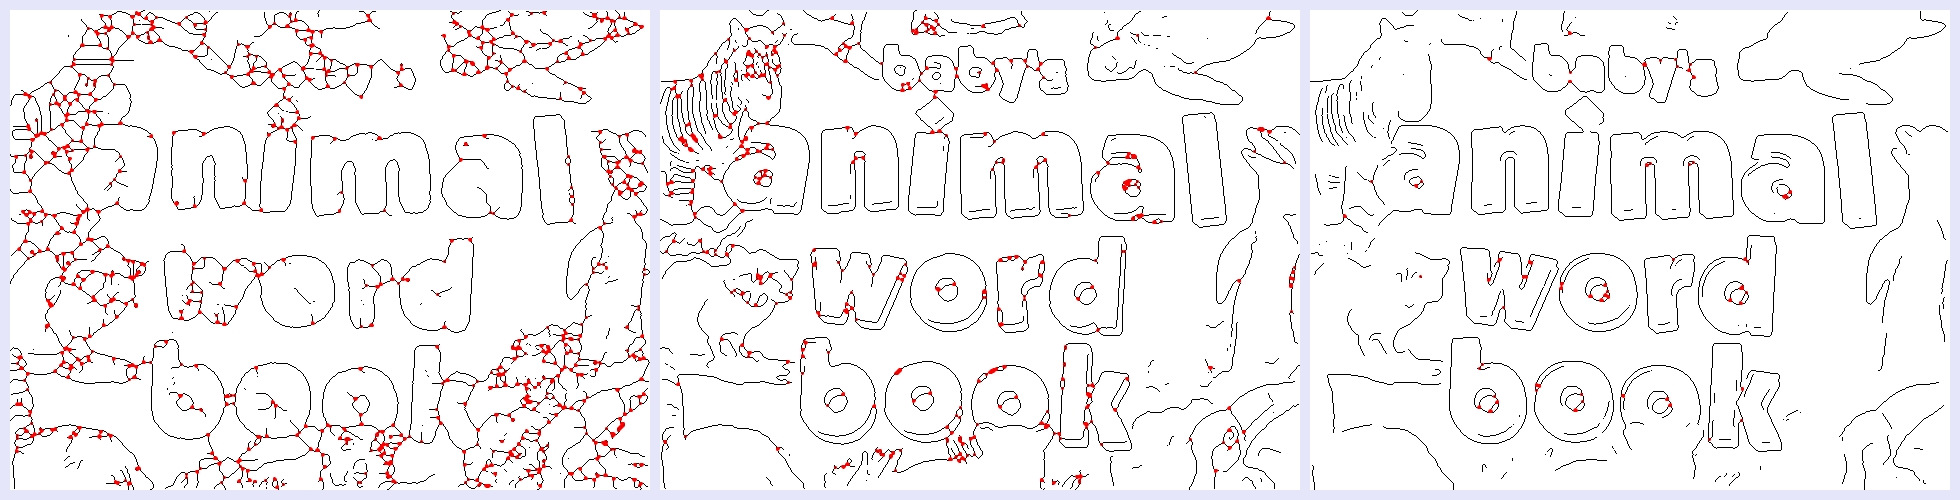
\includegraphics[width=\textwidth]{./figures/c3_compare_skeleton.jpg}
        \caption{不同的边缘骨架图的连通区域数目稳定,但孔洞数目变化剧烈}
        \label{fig.c3_compare_skeleton}
        \end{figure*}

        欧拉数是二值图像的拓扑特征,其数值是连通区域数目与孔洞数目的差值。由不同的二值边缘图所生成的边缘骨架图,它们的连通区域数目比较稳定,但是孔洞数目的变化很剧烈。如图\ref{fig.c3_compare_skeleton} 所示,过低或过高的分割阈值下的二值边缘图所生成的边缘骨架图的孔洞数与连通区域的数目的差距很大,而正常分割阈值下的边缘骨架图中孔洞数目和连通区域数目的差值则保持在合理范围内。

        1种简单且有效的计算欧拉数的方法是计算$2*2$ 像素模式的数目,这些像素模式的类型存在以下几类:

        $Q_1 = \left\{
        \quad
        \begin{matrix} 1 & 0 \\ 0 & 0 \end{matrix}\quad,\quad
        \begin{matrix} 0 & 1 \\ 0 & 0 \end{matrix}\quad,\quad
        \begin{matrix} 0 & 0 \\ 0 & 1 \end{matrix}\quad,\quad
        \begin{matrix} 0 & 0 \\ 1 & 0 \end{matrix}
        \quad
        \right\}$

        $Q_2 = \left\{
        \quad
        \begin{matrix} 0 & 1 \\ 1 & 1 \end{matrix}\quad,\quad
        \begin{matrix} 1 & 0 \\ 1 & 1 \end{matrix}\quad,\quad
        \begin{matrix} 1 & 1 \\ 1 & 0 \end{matrix}\quad,\quad
        \begin{matrix} 1 & 1 \\ 0 & 1 \end{matrix}
        \quad
        \right\}$

        $Q_3 = \left\{
        \quad
        \begin{matrix} 0 & 1 \\ 1 & 0 \end{matrix}\quad,\quad
        \begin{matrix} 1 & 0 \\ 0 & 1
        \end{matrix}
        \quad
        \right\}$

        其中,$Q_1$为外角点,$Q_2$ 为内角点,$Q_3$ 为交叉点,这些角点在边缘骨架上的位置如图\ref{fig.c3_select_skeleton}(b) 所示。那么欧拉数目的计算可由公式\ref{eq:c3_euler_number} 得到:

        \begin{equation}
        \eta=\frac{n(Q_1)-n(Q_2)+2n(Q_3)}{4},
        \label{eq:c3_euler_number}
        \end{equation}

        接下来,只有欧拉数和粘连点数最合适的边缘骨架图被保留下来,其它的边缘骨架图全部被删去。通过上述方式选择出来的边缘骨架图,既避免了过高分割阈值下的边缘图所可能生成的碎片和断裂化的边缘骨架,又避免了过低分隔阈值时可能生成的孔洞过多的杂乱边缘骨架,且因为删去了绝大多数无效的候选边缘骨架,而节省了计算量和时间。最后,将最合适的边缘骨架图上的粘连点消除掉,即可以将候选文字边缘骨架从背景中分离出来,以此来解决边缘粘连问题。

    \section{非文字骨架的滤除}
    \esection{Non-text skeleton's filtering}

    在\ref{sec.c3_skeleton}节中,我们论述了边缘骨架的生成方法,而在\ref{sec.c3_skeleton_cut} 节阐明了从背景中分隔出候选文字边缘骨架的具体步骤。目前,所有候选文字边缘骨架与非文字的边缘骨架之间的粘连点已经断裂开来,因此边缘粘连问题被解决了。但是在这些候选的边缘骨架中,还混杂有一些非文字的边缘骨架,需要被分类判别出来并清楚掉。所以在本节,提出1 个两阶段的文字边缘骨架分类方法,用以滤除掉混杂在文字边缘骨架中的非文字边缘骨架杂质。

        \subsection{形态学滤除}
        \esubsection{Morphological filtering}

        第1阶段的分类方法是形态学滤除。首先,从图\ref{fig.c3_compare_skeleton}(a) 和图\ref{fig.c3_compare_skeleton}(b) 的对比中,我们可以分析出文字边缘骨架和非文字边缘骨架之间在形态上的不同:背景边缘骨架比较直且分散,而文字边缘骨架则相对而言弯曲且聚合在一起。基于这一观察,大量的非文字边缘骨架就可以通过一些形态学的限制来过滤掉。

        \begin{figure*}[!h]
        \centering
        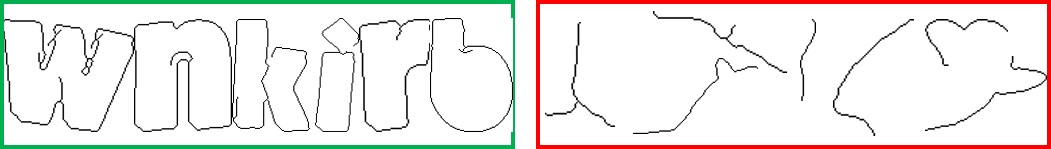
\includegraphics[width=\textwidth]{c3_skeleton_samples.jpg}
        \begin{minipage}[t]{0.48\linewidth}
        \centerline{\small (a)文字边缘骨架}
        \end{minipage}
        \begin{minipage}[t]{0.48\linewidth}
        \centerline{\small (b)非文字边缘骨架}
        \end{minipage}
        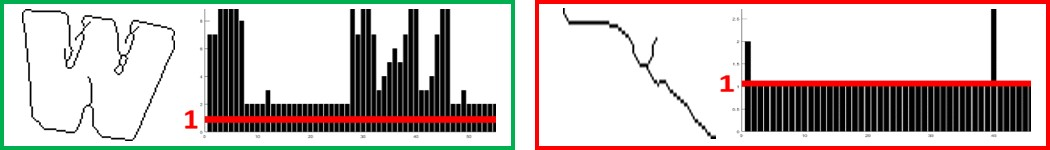
\includegraphics[width=\textwidth]{c3_concentration_ratio.jpg}
        \centerline{\small (c) 文字通常比非文字骨架具有更高的聚合度}
        \caption{文字与非文字边缘骨架的聚合度的比较} \label{fig.c3_concentration_ratio}
        \end{figure*}

        这些常用的形态学的限制包括:宽高比,离心率,欧拉数,同时在区域和其最小凸多边形中的像素比例,等等。而在本文中,针对文字边缘骨架和非文字边缘骨架的不同,提出一种简单但高效的形态学限制,即边缘骨架的聚合程度。假设给定边缘骨架$skel$,求取该边缘骨架的聚合度的方式如公式\ref{eq:c3_concentration_ratio} 所示:

        \begin{equation}
        C(skel)=\frac{length(skel_{ol})}{length(skel)},
        \label{eq:c3_concentration_ratio}
        \end{equation}

        其中,$skel_{ol}$是边缘骨架$skel$ 重叠的部分,即$skel_{ol}=skel(sum_{ver}(skel)>1)$。 而$Sum_{ver}(skel)$ 是按竖直方向将边缘骨架$skel$ 累加起来,如图\ref{fig.c3_concentration_ratio}(c) 所示:红线代表竖直方向累加像素点的个数为1 的阈值线,那么超过红线的位部分,表示该位置上存在重叠的边缘骨架$skel_{ol}$,即在$skel_{ol}$ 中 $Sum_{ver}(skel)>1$。 通过对图\ref{fig.c3_concentration_ratio}(c) 的观察,文字边缘骨架绝大部分都是重叠的,也就是$skel_{ol}$ 的长度占$skel$ 长度的比率$C(skel)$ 较大,因此较大的比率$C(skel)$ 表征了文字边缘骨架具有更高的聚合度。与此同时,观察发现非文字边缘骨架只有很小一部分是重叠的,即$skel_{ol}$ 的长度占$skel$ 长度的比率$C(skel)$ 很小,所以小$C(skel)$ 表征了非文字边缘骨架的聚合度更小。

        通过在第1阶段分类过程中,采用上述的这些简单的形态学限制,包括本文新提出的针对文字边缘骨架特征的聚合度限制,绝大多数非文字的边缘骨架就可以被高效的过滤掉。但是可能存在一些与文字边缘骨架极为相近的非文字边缘骨架没有在形态学过滤阶段被排除。那么这些被遗漏的非文字边缘骨架,就将在后续的第2 阶段分类过程中进行过滤。

        \subsection{基于卷积神经网络的滤除}
        \esubsection{convolutional neural network-based filtering}

        第2阶段的分类过程是更为精细的分类操作。受Wang 等\cite{Wang2012End} 提出的利用卷积神经网络(CNN) 作端对端文字识别方法的启发,在精细分类阶段我们提出一种基于CNN 的文字边缘骨架分类器,用于滤除掉遗漏下来的非文字边缘骨架。这个基于CNN 的边缘骨架分类器的架构如图\ref{fig.c3_cnn}所示,其网络结构是由2 个卷积层,分别后接2 个池化层,最后连1 个全连接层构成。其中第1 个卷积层有$n_1 = 64$ 个卷积模板,第2 个卷积层有$n_2 = 128$ 个卷积模板。全连接层后接2 个类别,分别为文字边缘和非文字边缘类别。2 类中置信度更高的类别即为分类判别结果。

        \begin{figure*}[!h]
        \centering
        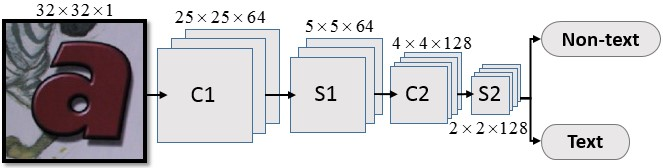
\includegraphics[width=\textwidth]{c3_cnn.jpg}
        \caption{单尺度卷积神经网络分类器的架构} \label{fig.c3_cnn}
        \end{figure*}

        这个CNN网络结构的输入是例如图\ref{fig.c3_cnn} 中最左边的小图块。这些小图块,是由经过第1阶段分类后被判别为候选文字边缘骨架的包围框,在原图上截取下来的小图块组成。在训练阶段,将这些图块的大小调整成$32 \times 32$ 个像素大小的训练样本,输入到CNN 网络中。然后在第1 个卷积层中,得到$25 \times 25 \times n_1$ 个卷积响应。接着在平均池化层,将响应的维度缩减到$5 \times 5 \times n_1$。 类似地,经过第2 个卷积层和池化层处理后,得到$2 \times 2\times n_1$ 的响应,并全连接到最后的分类层。训练网络时用squared hinge loss 作为损失函数。

        而在测试阶段,首先用基于Skeleton-cut 的文字边缘骨架检测子来生成候选的文字边缘骨架集合$P$,以及这些文字边缘骨架相对应的包围框集合$B$。 与Wang 等\cite{Wang2012End} 方法中利用滑动窗在原图的多尺度金字塔图像中扫描全图来计算卷积和池化响应不同,本文中要进行卷积处理的图块既不需要扫描全图,也不用因为考虑多尺度文字而在原图的多尺度金字塔图像上扫过滑动窗。本文只要对候选文字边缘骨架集合$B$ 中的每个边缘骨架的图块作分类判别即可,并且对这些图块只需作单尺度$s = height(B)$ 的变化。因此相比较过去的基于滑动窗的CNN 分类判别器而言,本文中利用CNN 进行文字与非文字边缘骨架分类的方法要更为高效和省时。

        最终,经过2层卷积和池化的响应输入到SVM 分类器,由此得到候选文字边缘骨架集合$P$ 中每个候选边缘骨架$p$ 的分类分数。这其中,具有较低文字分类置信度的候选文字边缘骨架将会被删除。那么经过第2阶段过滤后,保留下来的文字边缘骨架包围框的集合$B$ 就是基于边缘骨架切割的文字检测方法的结果。集合$B$ 中的每个文字边缘骨架包围框都有自己相应的分类置信度成绩$C$。

    \section{文本行的局部迭代优化}
    \esection{Text line's iteratively local refinement}

    本文上述所提出的基于边缘骨架切割的检测方法和2 阶段分类判别方法可以获得较高的文字检测查全率,但是文字检测结果同真实结果值(ground truth)之间的重叠率还是不满足期望。为了达到文字检测过程中的紧凑性(compactness) 标准,我们通过下面的算法\ref{alg:c3_iter_local_refine} 来调整文字检测包围框,使其更靠近文字的真实位置:

    \begin{algorithm}[!h]
	\renewcommand{\algorithmicrequire}{\textbf{输入:}}
	\renewcommand{\algorithmicensure}{\textbf{输出:}}
	\caption{文本行的局部迭代优化算法}
	\label{alg:c3_iter_local_refine}
	\begin{algorithmic}[1]
		\REQUIRE 候选文字边缘骨架的包围框集合 $B$, 以及求取的MSER 集合 $M$
		\ENSURE 经过局部迭代优化操作,对定位调整后的包围框集合 $R$
		\STATE 将MSER集合$M$按照位置分成2 类:强MSER 子集合$S$,是指包含在$B$ 边界内部的MSER 集合;弱MSER 子集合$W$ ,是指位于$B$ 边界之外的MSER 集合
        \FOR {$b \in B$}
        \STATE //本算法的目的是:在文本行方向上,将$b$ 调整为$b_{exp}$
        \STATE 计算位于$b$中的MSER$S$ 的特征均值$ms$
		\REPEAT
        \STATE $ws:=\left\{ w \in W |\,ol(b_{exp},w)>T_{ol}, | yc_{ms}-yc_w|<T_{yc} \right\}$
        \STATE $rs:=\left\{ w \in ws |\,Dist_{h,w,sw,c}(ms,w)<T_{h,w,sw,c} \right\}$
        \STATE $S:=S\cup rs,W:=W / rs$
        \UNTIL{$rs=\varnothing$}
        \STATE $R:=B \cap S$
        \ENDFOR
	\end{algorithmic}
    \end{algorithm}

    其中,$Dist_f(s,w)$指的是$s_f$ 和$w_f$ 之间归一化的$L2$ 距离。而$f$ 是候选MSER 的特征,这些特征包含:$sw$ 是笔划宽度,$c$ 是HSV 和灰度的颜色通道,$h,w$是候选MSER的高度和宽度;$yc$ 是候选MSER 在y 坐标轴上的中心坐标;另外函数$ol$用以计算2 个候选MSER 的包围框之间的重叠率;而$T$ 是经过实验计算得出的经验阈值。

    \begin{figure*}[!h]
    \centering
    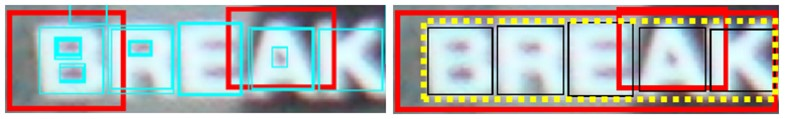
\includegraphics[width=\textwidth]{c3_iter_local_refine.jpg} \caption{局部迭代优化的效果示例}
    \label{fig.c3_iter_local_refine}
    \end{figure*}

    利用局部迭代优化方法来矫正文本行的实验效果如图\ref{fig.c3_iter_local_refine} 所示:图中左边的是未经过局部迭代优化前的文字检测结果,其中用红色矩形框标注的是用基于边缘骨架切割的检测子提取出的候选文字,用蓝色矩形框标注的是用MSER 提出的候选文字;而图中右边的是经过局部迭代优化后得到的文字检测结果,可看出通过算法\ref{alg:c3_iter_local_refine} 将基于边缘骨架切割的文字检测子和基于MSER 的检测方法结合起来,从而追回那些因图像模糊而未被检测到的候选文字。通过文本行局部迭代优化后得到的最终检测结果如图\ref{fig.c3_iter_local_refine} 中右图内的黄色虚线包围框所示,可见包围框的查全率以及同真实结果值之间的重叠率都得到了极大提升。

    \section{实验和结果分析}
    \esection{Experimental Results}

        \subsection{实验数据集与评价标准}
        \esubsection{Data-set and Evaluation Protocol}

        为了验证本章提出的文字检测子的效果,将该检测子运行在自然场景文字测试集ICDAR 2013 上。这个测试集合包含462 张标注的自然场景文字图片,其中有229 张图片用以训练,而233 张图片用于测试。该测试集合非常具有挑战性:因为图片存在光照不均、尺度不同(尺度范围从$459 \times 405$ 到$3888 \times 2592$) 的问题,而且文字也存在不同字体和颜色的问题。此外还利用了MSRA-TD500 测试数据集来验证本方法在多方向和多语种文字图像样本上的检测效果。最终使用Wolf 等\cite{Wolf2006Object} 提出的评价标准来验证本方法的文字检测结果。评价标准利用到了查全(recall),查准(precision) 和f 值等概念,这些概念来源于信息检索领域(Information Retrieval,IR)。

        其中查全率(recall)代表的含义是真值(ground truth)中的东西被提取出来的比例:
        \begin{equation}
        recall=\frac{N.o. \quad True Positives}{N.o. \quad Ground truth}
        \end{equation}

        而查准(precision)表示检测到的东西是正确的比例:
        \begin{equation}
        precision=\frac{N.o. \quad True Positives}{N.o. \quad Retrieved Items}
        \end{equation}

        其中,符号N.o是数量Number of 的首字母缩写。最后综合指标F-mean (也可记为F-score)是查全(recall)和查准(precision)的调和平均数(Harmonic mean),该指标用以衡量算法的综合性能:
        \begin{equation}
        F=\frac{2}{\frac{1}{recall}+\frac{1}{precision}}=\frac{2recall*precsion}{recall+precision}
        \end{equation}

        文字检测算法也会引入查全和查准来衡量算法性能,但存在3 项复杂性:

        1)文字或目标检测与信息检索(IR)的不同:设文字检测方法结果和真值(ground truth)中的定位包围盒(bounding box)分别用$D_i$ 和$G_j$ 表示,那么就判断$D_i$ 是否为true positive而言,文字检测要比信息检索(IR)更为困难。这是因为在文字检测中,存在1个$D_i$ 和多个$G_j$ 匹配的情况,因此其用作正确性判断的匹配方法是soft (匹配值是由0 到1 之间的1 个分数)和非一对一的匹配。

        2)文字检测与目标检测也存在差异:首先,文字可以在字符、单词或文本行这几个层级(或称为粒度)上进行衡量;然后对于文字检测问题来说,其最终目标是为文字识别提供精准的输入,并且检测结果能极大程度地决定识别效果。

        因此对于文字检测的评判要比一般目标检测更为严格。而在计算查全和查准时的关键是决断两个文字定位包围盒是否匹配。如图\ref{fig.c3_evalu_bbox_match}所示,总共存在3 种匹配的方式:

        \begin{figure*}[!h]
        \centering
        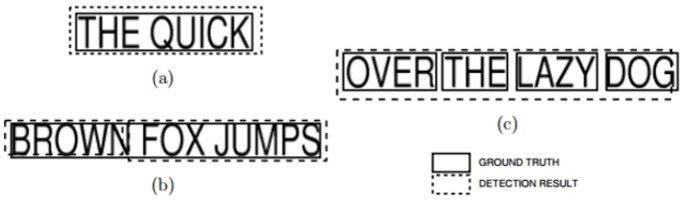
\includegraphics[width=\textwidth]{c3_evalu_bbox_match.jpg} \caption{文字检测区域结果(detection result)与真实区域(ground turth)之间的匹配状况:图(a) 是1对1 的匹配示例;图(b)1 对多的匹配示例;图(c)是多对1 的匹配示例}
        \label{fig.c3_evalu_bbox_match}
        \end{figure*}

        其中ICDAR2003数据集采用的就是1对1的匹配方式\cite{Mariano2002Performance},这种匹配方式最为简洁,其计算过程如公式\ref{eq.c3_match_1v1}所示:

        \begin{equation}
        \left\{
        \begin{array}{c}
        R(G,D)=\frac{\sum_{i=1}^GBestMatch_G(G_i)}{|G|}\\
        P(G,D)=\frac{\sum_{j=1}^DBestMatch_D(D_j)}{|D|}
        \end{array}
        \right.
        \label{eq.c3_match_1v1}
        \end{equation}
        
        

        \subsection{实验结果与分析}
        \esubsection{Experimental Results and Analysis}

        如表\ref{tab.c3_icdar13}所示,本章提出的方法在ICDAR 2013 测试数据集上取得了86.79\%的查准率和76.21\%的查全率。该方法的查全率超过了其它所有的检测方法的查全率,这得益于文字边缘骨架提取方法的良好设计。同时我们提出了2 阶段非文字过滤以及文本行的局部迭代优化策略,以确保本方法的高查准结果。值得一提的是,本方法没有使用传统的图像金字塔上的多尺度滑动窗进行文字与背景的二分类,而是采用文字边缘骨架提取加单尺度的CNN分类判断,因此在保证检测成绩的同时,大幅缩减了计算量和用时。另外,在提出的方法中融入文本行的局部迭代优化(Iteratively Local Refinement,简称ILR),可以进一步将检测F 值提升3.3\%,并超越其它所有先进的文字检测方法。

        \begin{table*}[!h]
        \centering
        \caption{在ICDAR 2013上的文字检测效果(\%)}
        \begin{tabular}{p{0.25\textwidth}|p{0.25\textwidth} p{0.25\textwidth} p{0.13\textwidth}}
        \hline
        方法 & 查全R & 查准P & F值 \\
        \hline
        \textbf{Proposed} & \textbf{76.21} & \textbf{86.79} & \textbf{81.16}(+3.3) \\
        Without \textbf{ILR} & 73.28 & 84.80 & 77.83 \\
        \hline
        Tian\cite{Tian2016Text} & 75.89 & 85.15 & 80.25 \\
        Zhu\cite{Zhu2016Text} & 75.00 & 85.00 & 79.00 \\
        Gupta\cite{Gupta2016Synthetic} & 66.30 & 94.80 & 78.00 \\
        Yin\cite{Yin2013Robust} & 65.11 & 83.98 & 75.89 \\
        Neumann\cite{Neumann2012Real} & 64.84 & 87.51 & 74.49 \\
        \hline
        \end{tabular}
        \label{tab.c3_icdar13}
        \end{table*}

        表格\ref{tab.c3_icdar11}展示了本方法与若干先进方法在ICDAR 2011测试数据集上关于字符检出率的量化比较。ICDAR 2011测试数据集包含255 张自然场景图片,里面总共有6309个字符。在进行对比的几种方法中,若对提取到的所有极值区域(Extremal Region,简称为ER) 都不判别而直接认定为字符,那么字符的检出率高达96\%。但这样的话提取的候选字符有6 百万之多,计算量过大,并且在这么多的候选字符中真正的字符更难被提取出来,因而查准率极低。如果采用Matas 等\cite{Matas2004Robust} 提出的最稳定极值区域(Maximally Stable Extremal Regions,简称为MSER),则候选字符数目骤降到3 万个,计算量大幅下降,且查准率得到提升。但从检出率的指标来看,该方法的成绩也从96\% 减低到53\%,因此牺牲的是文字检测的查全效果。

        \begin{table*}[htbp]
        \centering
        \caption{在ICDAR 2011测试集上对于字符提取数目和检出率的测评}
        \begin{tabular}{p{0.33\textwidth}|p{0.33\textwidth} p{0.25\textwidth}}
        \hline
        方法 & 候选字符数目 & 检出率 \\
        \hline
        All ERs & 6,051,331 & 0.966 \\
        \hline
        Matas\cite{Matas2004Robust} & 39,762 & 0.539 \\
        \hline
        Sung\cite{Sung2015Scene} &  &  \\
        Initial ERs & 1,729,833 & 0.896 \\
        Refined ERs & 93,357 & 0.877 \\
        \hline
        \textbf{Our method}  &  &  \\
        Initial Skeletons & 608,394 & 0.936 \\
        + Classifier & 6,034 & 0.842 \\
         + Classifier + ILR & 8,231 & 0.879 \\
        \hline
        \end{tabular}
        \label{tab.c3_icdar11}
        \end{table*}

        在候选字符数目与字符检出率的折衷方面做的较好的是Sung 等\cite{Sung2015Scene} 提出的方法。这个方法首先在提取极值区域ER 的初始阶段保证了89\% 的高检出率,同时候选字符的数目也维持在较低的水平。接着在后续阶段此方法继续大幅降低候选字符的数量直到9 万多个,而检出率也仅下降了2\% 而已。从结果上来看,Sung 的方法可以说既保证了文字检查的高查全率,同时还兼顾了检出文字的高水平查准效果。而本章提出的方法进一步加大了这种高查全兼顾高查准的优势:在使检出率高于Sung 的方法的同时,又使候选字符的数目相对于Sung 的方法降低了1 个量级。因此从在ICDAR 2011 测试集上的字符检测结果来说,本章提出方法优于其它先进的文字检测方法。

        \begin{table*}[!h]
        \centering
        \caption{ 本方法与其它文字检测方法在MSRA-TD500 测试数据集上的检测成绩对比}
        \begin{tabular}{p{0.25\textwidth}|p{0.25\textwidth} p{0.25\textwidth} p{0.13\textwidth}}
        \hline
        方法 & 查全R & 查准P & F值 \\
        \hline
        \textbf{Proposed} & 0.64 & 0.82 & 0.72 \\
        Yin\cite{Yin2015Multi} & 0.63 & 0.81 & 0.71 \\
        Kang\cite{Kang2014Orientation} & 0.62 & 0.71 & 0.66 \\
        Yin\cite{Yin2013Robust} & 0.61 & 0.71 & 0.65 \\
        Tu\cite{Tu2012Detecting} & 0.63 & 0.63 & 0.60\\
        \hline
        \end{tabular}
        \label{tab.c3_msra}
        \end{table*}

        如表格\ref{tab.c3_msra}所示,我们的方法还与其它方法在微软MSRA-TD500 文字检测数据集上进行了对比。本章提出的方法取得了查全0.64,查准0.82 以及F 值0.72 的检测结果,其成绩显著高于其它方法。微软MSRA-TD500 数据集中的文本大多倾斜、弯曲并由多国语言构成。而从MSRA-TD500 的实验结果上来看,本方法可以在自然场景图像中成功检测到多方向和多语种的文本。

        \begin{figure}[!h]
        \centering
        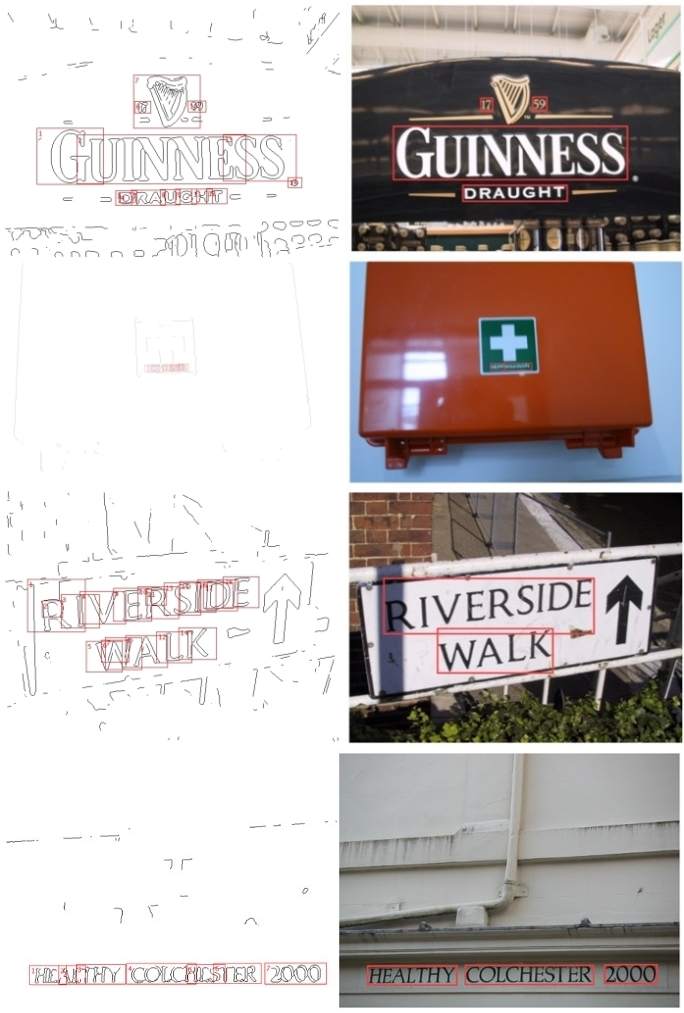
\includegraphics[width=\textwidth]{c3_ic13_results.jpg}
        \caption{ICDAR2013 上的测试结果示例}
        \label{fig.c3_ic13_results}
        \end{figure}

        \begin{figure}[!h]
        \centering
        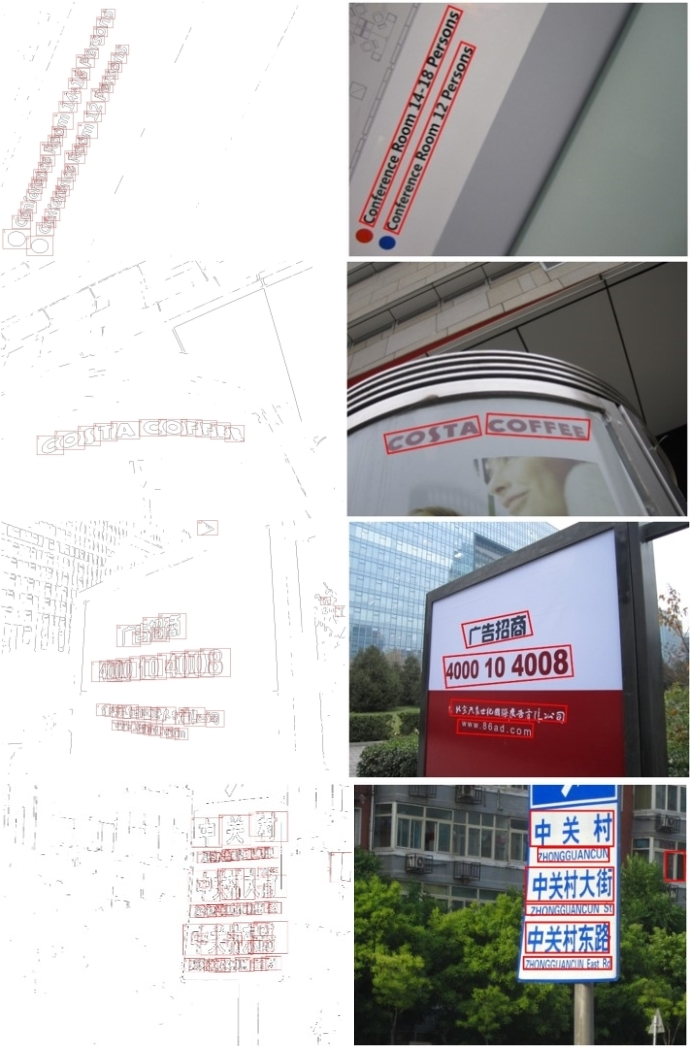
\includegraphics[width=\textwidth]{c3_msra_results.jpg}
        \caption{MSRA-TD500 上的测试结果示例}
        \label{fig.c3_msra_results}
        \end{figure}

    \section{本章小结}
    \esection{Brief Summary}

    本章提出的是基于边缘骨架切割的文字检测方法。首先对于输入的场景文字图片,利用结构化边缘检测方法得到边缘响应图,然后基于一系列像素强度值阈值,对边缘响应图进行分割,得到相应的二值化边缘图。接着在每个二值边缘图上,通过细化操作得到其边缘骨架图,并通过8 领域内像素点分析所找到的边缘骨架结点。而文字边缘与背景间的粘连点,就存在于这些边缘骨架结点中。因此断开粘连点得到候选的文字边缘骨架,然后经过形态学滤除来过滤掉大部分明显不是文字的边缘骨架,剩余的不易区分的非文字边缘骨架,可通过基于 CNN 的分类器来进一步滤除。最后基于非极大值抑制和文本行聚集操作,得到文本行定位结果。

    在公开数据集ICDAR2011,ICDAR2013以及MSRA-TD500 上,我们对本章提出的方法都进行了实验,并将实验结果与其它先进方法进行了比较。实验结果证明了该方法的有效性。此外通过分析本章提出的方法,以及针对其文字定位包围盒不够精准的局限,我们将会在下一章中提出基于二叉树搜索的文本行优化方法。


